\subsection{Caso randomico}

Confrontiamo adesso i due metodi ponendo in ingresso numerosi valori pseudo-casuali e osserviamo come si comportano le tabelle di conseguenza.

\begin{figure}[p]
\centering
\subfloat{%
  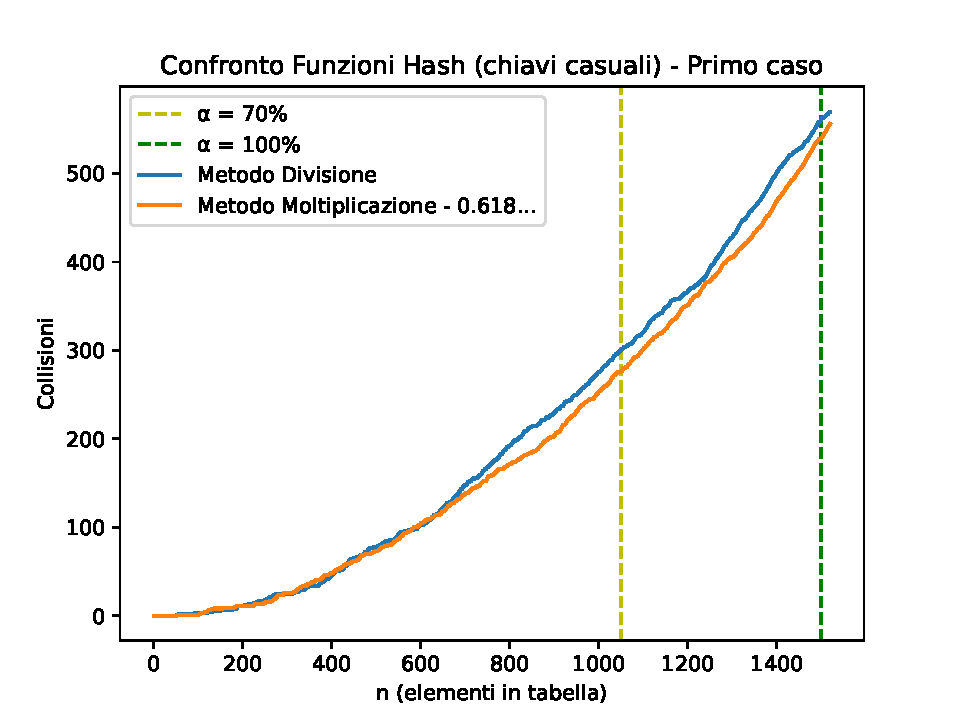
\includegraphics[width=0.67\textwidth]{src/img/CASO1.pdf}%
  } \\
\subfloat{%
  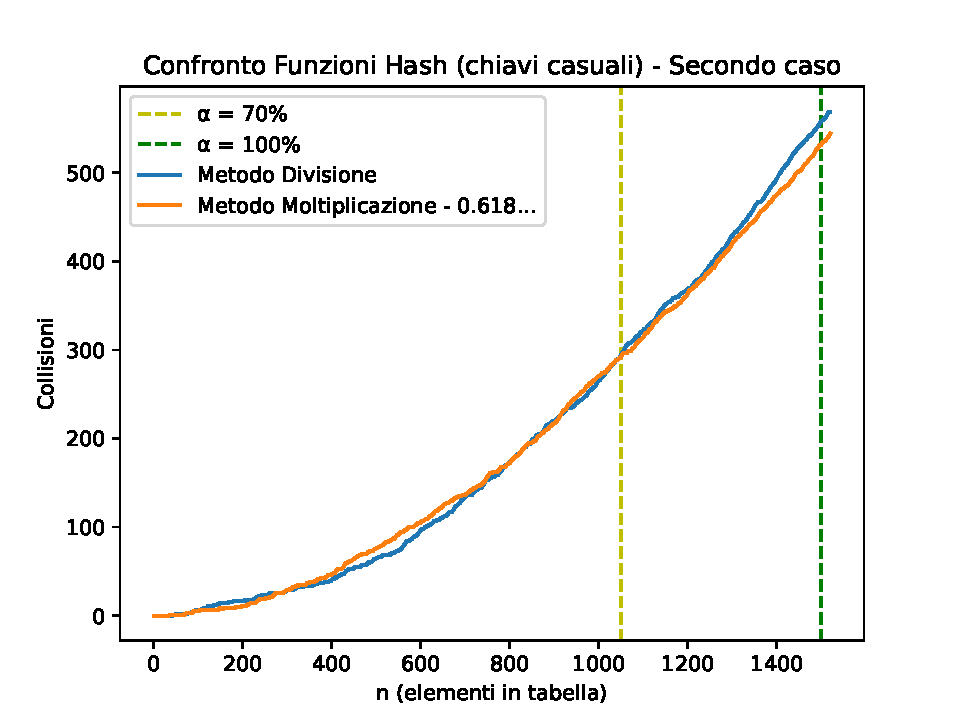
\includegraphics[width=0.68\textwidth]{src/img/CASO2.pdf}%
  }   \\     
\subfloat{%
  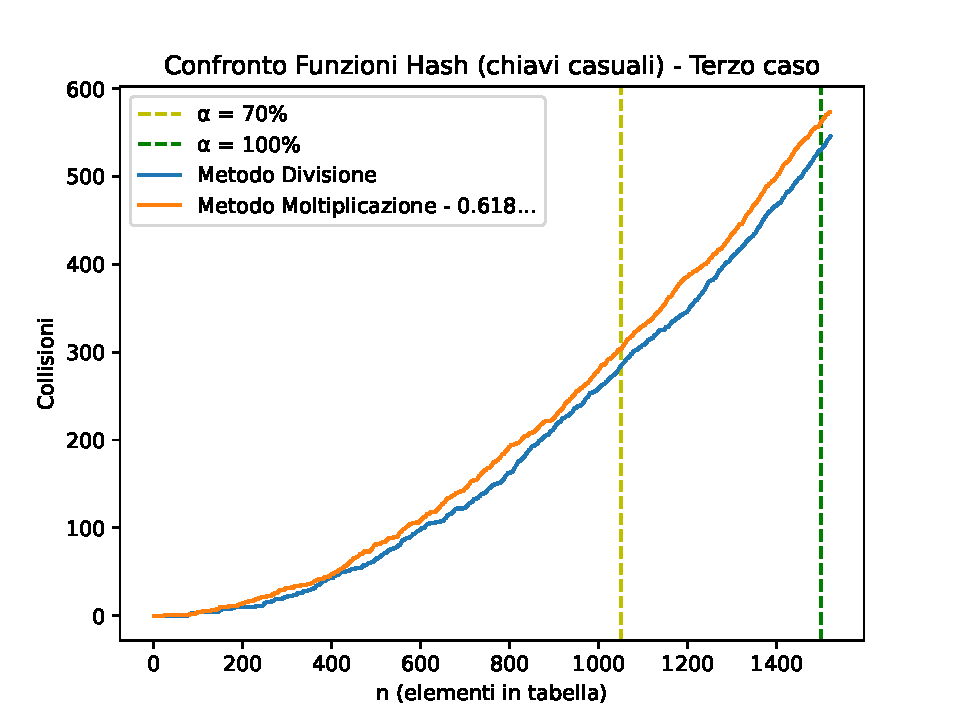
\includegraphics[width=0.68\textwidth]{src/img/CASO3.pdf}%
  } 
\caption{I tre casi a confronto}
\label{fig:random_casi}
\end{figure}

In tutti e tre gli scenari, abbiamo $m = 1500$ e un universo delle chiavi pari a $m \cdot 20=30000$, quindi molto ampio.
Per generare i numeri casuali, sono stati inseriti tutti i numeri da $1$ fino a $m\cdot20$ in una lista sfruttando la funzione \verb|list(range(1,m*20))|, che è stata poi mescolata con la funzione \verb|shuffle| della libreria \verb|random|.
Infine sono stati effettivamente inseriti in tabella i primi $m+20$ elementi\footnote{Un valore a piacimento di poco superiore a $m$ per vedere l'evoluzione della tabella fino (e oltre) $\alpha=100\%$}.
Lo snippet di riferimento è il seguente:
% multiline code snippet
\lstset{
      basicstyle=\small,
      xleftmargin=.1\textwidth,
}
\begin{lstlisting}
tot_ele = m+20
key_universe = list(range(1,m*20))
random.shuffle(key_universe)

for i in range(tot_ele):
	Hash.insert(User(key_universe[i]-1, "i"))
\end{lstlisting}

\textit{Nota}: l'attributo \verb|value| è semplicemente l'indice dell'elemento all'interno della lista (non ha molta importanza).

Passiamo dunque a commentare quanto ottenuto, che è riportato graficamente in Figura \ref{fig:random_casi}.
Notiamo subito la cosa più importante: l'andamento in tutti e tre i (sotto)casi è \textit{simile}: dei due metodi non ce n'è uno predominante. Entrambi causano all'incirca lo stesso numero di collisioni.
\\In dettaglio nel \textit{Primo caso} il metodo della divisione appare leggermente svantaggiante, soprattutto dopo un certo elemento di valori inseriti.
\\ Situazione sostanzialmente di "pareggio" invece nel \textit{Secondo caso}, con i due metodi che in termini di collisioni praticamente si equivalgono.
\\ Infine nel \textit{Terzo caso} risulta lievemente meno performante il metodo della moltiplicazione, nonostante sia stato impostato ad $A$ il valore di Knuth.

Importante sottolineare che se eseguiamo più e più volte il programma, ci ritroviamo sempre in uno dei tre contesti appena esposti, il che ci fa riflettere ancora una volta sull'efficacia e sulle differenze dei metodi. Il tutto sarà descritto completamente nella sezione successiva delle Conclusioni.